\documentclass[a4paper]{article}
\usepackage{forest}
\usepackage{float}
\usepackage{makecell}
\usepackage{geometry}
\usepackage{listings}
\usepackage{hyperref}
\usepackage{graphicx}
\usepackage{ragged2e}
\usepackage{color}
\usepackage{xepersian}
\usepackage{subfiles}
\newgeometry{left=1.4cm, right=1.4cm, bottom=2.0cm, top=2.0cm}
\settextfont[Scale=1]{XB Roya}

\title{سند ۴+۱ در معماری نرم‌افزار}
\author{علیرضا سلطانی نشان}

\begin{document}
\maketitle

در سال ۱۹۹۵ آقای \lr{Philippe B.Kruchten} مقاله‌ای را تحت عنوان \lr{Software
Architecture} منتشر کرد که در بند اول آن نوشته بود \cite{kruntchen1995architectural}:

معماری نرم‌افزار در سطح بسیار بالایی از تجرید قرار دارد و طراحی منطقی یک
نرم‌افزار می‌باشد در حالی که طراحی نرم‌افزار کمترین مقدار تجرید را دارد و تمام
جزئیات المان‌ها و ارتباطاتشان با یکدیگر مشخص است و همچنین شامل طراحی فیزیکی نیز
می‌باشد.

آقای \lr{Kruchten} بر این باور است که نوشتن ایده‌ها بر روی کاغذ همیشه مفید خواهد
بود قبل از اینکه آن را کد کنیم. ایشون به صراحت مطرح می‌کند که همیشه مصور‌سازی
بهتر از خواندن مستندات کسل‌کننده است و در نهایت مهم‌ترین انگیزه برای تهیه سند
۴+۱ از نظر او آن است که مدل‌سازی آن آسان است زیرا باعث می‌شود که سیستم را از
دیدگاه‌های مختلفی بررسی کنیم.

ایده مدل معماری ۴+۱ برای رفع مشکل جمع شدن اطلاعات بیش از حد در یک نمودار معماری
نرم‌افزار یا عدم رسیدگی به برخی از نگرانی‌های ذینفعان بوده است تا بتواند تمام
جنبه‌ها را در ۴+۱ مدل در یک معماری نرم‌افزاری پوشش دهد.

\begin{table}[H]
    \centering
    \caption{تفاوت میان طراحی و معماری در نرم‌افزار \cite{medium}}
        \begin{tabular}{c|c}
            \textbf{معماری} & \textbf{طراحی} \\ \hline
            در سطح کل سیستم & در سطح هر ماژول و کامپوننت \\
            ویژگی‌های اصلی و اساسی & ویژگی‌های جزئی در سیستم \\
            سخت در ایجاد تغییرات به دلیل تاثیر در کل سیستم & آسان در ایجاد تغییر به دلیل \lr{Separation of Concerns}
        \end{tabular}
\end{table}

\section*{ویو‌های سند ۴+۱}

مدل \lr{View} ۴+۱ توصیفی از معماری نرم‌افزار را با استفاده از پنج \lr{View}
همزمان مدیریت و سازماندهی می‌کند که هر کدام از \lr{View}ها به مجموعه خاصی از
نگرانی‌ها می‌پردازد:

\begin{enumerate}
    \item \lr{Logical View}: تمام عملیاتی که سیستم می‌تواند به کاربران نهایی
    ارائه دهد را در این قسمت مدیریت خواهیم کرد که عموماً از نیازمندی‌های عملیاتی
    یا \lr{Functional requirements} تشکیل شده است و از نمودار‌های کلاس و
    کامپوننت می‌توانیم در آن کاربران و مدل‌هایشان را تعریف کنیم.
    \item \lr{Process View}: تمرکز اصلی آن بر تمام نیازمندی‌های غیرعملیاتی یا
    \lr{Non-functional requirements} در زمان اجرای سیستم است که شامل موارد،
    امنیت، کارایی بالا، در دسترس بودن، مدیریت همزمانی، و تحمل خطا
    \footnote{\lr{Fault-tolerance}} می‌باشد و از نمودار‌های \lr{Sequence} و
    \lr{Activity} برای نمایش آن‌ها استفاده می‌کنیم.
    \item \lr{Development View}: این ویو سیستم را از دیدگاه یک توسعه‌دهنده نشان
    می‌دهد و با مدیریت نرم‌افزار سر و کار دارد. عموماً در این ویو از نمودار‌های
    پکیج و کامپوننت استفاده می‌شود.
    \item \lr{Physical View}: توصیف نمود نرم‌افزار بر روی سخت‌افزار و ارتباطات
    فیزیکی بین کامپوننت‌ها را مطرح می‌کند. عموماً از نمودار \lr{Deployment} برای
    نمایش استفاده می‌شود.
    \item \lr{Scenarios}: توصیف رفتار سیستم از نظر یک کاربران نهایی‌ای که از این
    سیستم می‌خواهد استفاده کند را نشان می‌دهد که از نمودار \lr{Usecase} استفاده
    می‌کند. 
\end{enumerate}

\begin{figure}[H]
    \centering
    \caption{چهار ویو مورد استفاده برای نشان‌دادن و اعتبارسنجی نیازمندی‌های یک
    پروژه نرم‌افزاری با یکدیگر پیوند دارند که در ابتدا بایستی آن‌ها را ایجاد
    کنیم و سپس از نمودار‌های مناسب برای مصور‌سازی آن‌ها استفاده کنیم.
    \cite{kruntchen1995architectural}}
    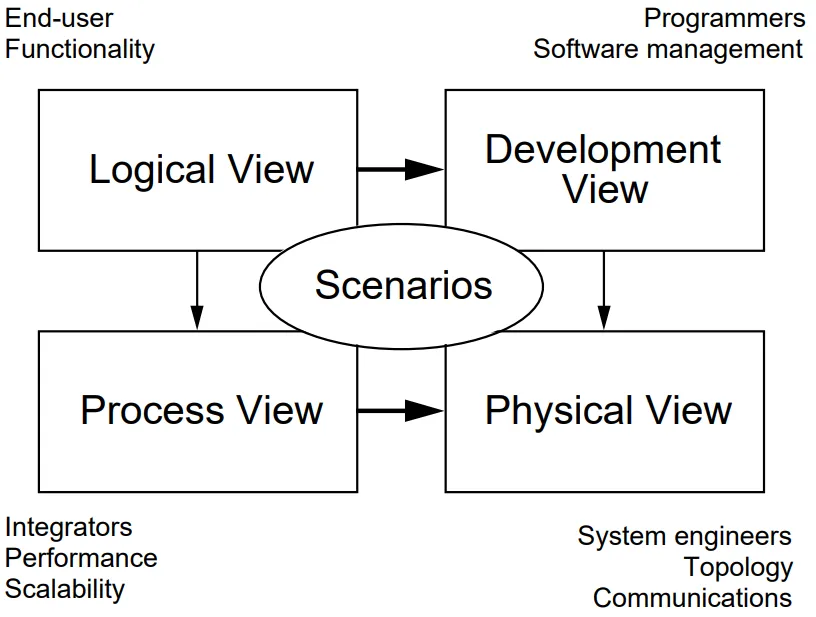
\includegraphics[width=0.8\textwidth]{diagrams/five_view.png}
\end{figure}

\section*{مزایا و معایب}

سند ۴+۱ به عنوان یک \lr{View model} دارای مزایا و معایبی زیر است \cite{linkedin}.

\subsubsection*{مزایا}

\begin{itemize}
    \item یک ساختار صریح و سازگار را به سازمان‌ها ارائه می‌دهد که به آن‌ها کمک
    می‌کند تا اطلاعات خود را مرتب و سازمان‌دهی کنند.
    \item این سند تمام دیدگاه‌های نسبت به سیستم را پوشش می‌دهد مانند
    نیازمندی‌های غیر-عملیاتی زیر:
    \begin{itemize}
        \item \lr{Functionality}
        \item \lr{Performance}
        \item \lr{Reliability}
        \item \lr{Scalability}
        \item \lr{Security}
        \item \lr{Deployment}
    \end{itemize}
    \item از سطوح چندگانه تجرید و جزئیات پشتیبانی می‌کند و به ذینفعان کمک می‌کند
    که روی \lr{View} که بیشتر ارتباط را به آن‌ها دارد تمرکز کنند.
    \item ارتباطات و همکاری بین تیم توسعه، مشتریان، مدیران، و تستر‌ها را از نظر
    استفاده از اصطلاحات \footnote{\lr{Terminology}} و \lr{Notation}ها بهتر
    می‌کند تا فهم بیشتری در گفت و گو‌ها داخلی بین گروه‌های مختلف بدست آید.
\end{itemize}

\subsubsection*{معایب}

\begin{itemize}
    \item این سند ممکن است با تمام سیستم‌ها یا دامنه‌ها، مناسب و \lr{Fit} نباشد.
    ممکن است به خاطر بعضی از جنبه‌های سیستم نیاز باشد که \lr{View}های مناسب نسبت
    به آن طراحی و دوباره تعریف شوند.
    \item به دلیل تغییرات سریع در سیستم مورد نظر در گذر زمان، ممکن است این سند
    وضعیت کنونی سیستم را نشان ندهد و برخی از قسمت‌های آن منسوخ شده و ناسازگار با
    سیستم جدید (در حال توسعه) باشد.
    \item ممکن است تمام تصمیمات طراحی و سبک سنگین‌هایی که
    \footnote{\lr{Trade-offs}} در طول فرایند توسعه رخ می‌دهد را در بر نگیرد چرا
    که ممکن است بعضی از آن‌ها به صورت ضمنی در جلسات باشند و حتی مستندسازی نسبت
    به آن انجام نشده باشد.
    \item این سند تلاش بسیار زیادی را برای مدیریت نیاز دارد تا بتواند ۵ لایه
    \lr{View} را نسبت به هم هماهنگ و منسجم نگه دارد به همین خاطر نگهداری و به
    روز رسانی آن کار آسانی نیست.
\end{itemize}

\section*{بررسی نهایی نمودار‌های مورد استفاده}

\begin{table}[H]
    \centering
    \caption{نمودار‌هایی که می‌توان در سند ۴+۱ متناسب با ویو استفاده کرد \cite{medium}.}
        \begin{tabular}{c|c}
            \textbf{نام ویو} & \textbf{دیاگرام \lr{UML}} \\ \hline
            \textbf{\lr{Logical view}} & \makecell{\lr{Class diagram}, \lr{Object diagram}, \lr{Component diagram} \\ \lr{Package diagram}, \lr{Composite Structure Diagram}} \\ \hline
            \textbf{\lr{Process view}} & \makecell{\lr{Activity diagram}, \lr{Sequence diagram}, \lr{Timing diagram} \\ \lr{State machine diagram}, \lr{Interaction overview diagram}} \\ \hline
            \textbf{\lr{Development view}} & \lr{Component diagram, Package diagram} \\ \hline
            \textbf{\lr{Physical view}} & \lr{Deployment diagram} \\ \hline
            \textbf{\lr{Scenarios}} & \lr{Usecase diagram} \\
        \end{tabular}
\end{table}

\section*{جایگزین‌ها}

اسنادی که می‌توانند به صورت جایگزین نسبت به سند ۴+۱ استفاده شوند به ترتیب زیر
هستند:

\begin{enumerate}
    \item سند \lr{C4}
    \item سند \lr{TOGAF}
    \item سند \lr{5+2}
    \item سند \lr{SysML}
    \item سند \lr{ArchMate}
    \item سند \lr{ADL}
\end{enumerate}

\newpage
\bibliographystyle{unsrt-fa}
\bibliography{kruchten_refs.bib}
\end{document}